\documentclass{article}\usepackage[]{graphicx}\usepackage[]{color}
%% maxwidth is the original width if it is less than linewidth
%% otherwise use linewidth (to make sure the graphics do not exceed the margin)
\makeatletter
\def\maxwidth{ %
  \ifdim\Gin@nat@width>\linewidth
    \linewidth
  \else
    \Gin@nat@width
  \fi
}
\makeatother

\definecolor{fgcolor}{rgb}{0.345, 0.345, 0.345}
\newcommand{\hlnum}[1]{\textcolor[rgb]{0.686,0.059,0.569}{#1}}%
\newcommand{\hlstr}[1]{\textcolor[rgb]{0.192,0.494,0.8}{#1}}%
\newcommand{\hlcom}[1]{\textcolor[rgb]{0.678,0.584,0.686}{\textit{#1}}}%
\newcommand{\hlopt}[1]{\textcolor[rgb]{0,0,0}{#1}}%
\newcommand{\hlstd}[1]{\textcolor[rgb]{0.345,0.345,0.345}{#1}}%
\newcommand{\hlkwa}[1]{\textcolor[rgb]{0.161,0.373,0.58}{\textbf{#1}}}%
\newcommand{\hlkwb}[1]{\textcolor[rgb]{0.69,0.353,0.396}{#1}}%
\newcommand{\hlkwc}[1]{\textcolor[rgb]{0.333,0.667,0.333}{#1}}%
\newcommand{\hlkwd}[1]{\textcolor[rgb]{0.737,0.353,0.396}{\textbf{#1}}}%

\usepackage{framed}
\makeatletter
\newenvironment{kframe}{%
 \def\at@end@of@kframe{}%
 \ifinner\ifhmode%
  \def\at@end@of@kframe{\end{minipage}}%
  \begin{minipage}{\columnwidth}%
 \fi\fi%
 \def\FrameCommand##1{\hskip\@totalleftmargin \hskip-\fboxsep
 \colorbox{shadecolor}{##1}\hskip-\fboxsep
     % There is no \\@totalrightmargin, so:
     \hskip-\linewidth \hskip-\@totalleftmargin \hskip\columnwidth}%
 \MakeFramed {\advance\hsize-\width
   \@totalleftmargin\z@ \linewidth\hsize
   \@setminipage}}%
 {\par\unskip\endMakeFramed%
 \at@end@of@kframe}
\makeatother

\definecolor{shadecolor}{rgb}{.97, .97, .97}
\definecolor{messagecolor}{rgb}{0, 0, 0}
\definecolor{warningcolor}{rgb}{1, 0, 1}
\definecolor{errorcolor}{rgb}{1, 0, 0}
\newenvironment{knitrout}{}{} % an empty environment to be redefined in TeX

\usepackage{alltt}

\usepackage{amsmath, amsthm, amsfonts}
\usepackage{enumerate}
\usepackage{hyperref}

\title{Assignment 2}
\author{Anh Le}
\IfFileExists{upquote.sty}{\usepackage{upquote}}{}
\begin{document}

\maketitle

\begin{knitrout}
\definecolor{shadecolor}{rgb}{0.969, 0.969, 0.969}\color{fgcolor}\begin{kframe}
\begin{alltt}
\hlcom{## knitr configuration: http://yihui.name/knitr/options#chunk_options}
\hlstd{opts_chunk}\hlopt{$}\hlkwd{set}\hlstd{(}\hlkwc{comment} \hlstd{=} \hlstr{""}\hlstd{,} \hlkwc{error}\hlstd{=} \hlnum{TRUE}\hlstd{,} \hlkwc{warning} \hlstd{=} \hlnum{FALSE}\hlstd{,} \hlkwc{message} \hlstd{=} \hlnum{FALSE}\hlstd{,}
               \hlkwc{tidy} \hlstd{=} \hlnum{FALSE}\hlstd{,} \hlkwc{cache} \hlstd{= F,} \hlkwc{echo} \hlstd{= T,}
               \hlkwc{fig.width} \hlstd{=} \hlnum{4}\hlstd{,} \hlkwc{fig.height} \hlstd{=} \hlnum{4}\hlstd{,} \hlkwc{fig.align}\hlstd{=}\hlstr{"center"}\hlstd{)}
\end{alltt}
\end{kframe}
\end{knitrout}


\section{Question 1}

Let's pursue further the in-class example of ordering / selecting one variable based on another. We have the following mock data.
\begin{knitrout}
\definecolor{shadecolor}{rgb}{0.969, 0.969, 0.969}\color{fgcolor}\begin{kframe}
\begin{alltt}
\hlstd{mock_data} \hlkwb{<-} \hlkwd{data.frame}\hlstd{(}\hlkwc{country}\hlstd{=}\hlkwd{c}\hlstd{(}\hlstr{"US"}\hlstd{,} \hlstr{"UK"}\hlstd{,} \hlstr{"South Africa"}\hlstd{,} \hlstr{"Liberia"}\hlstd{),}
                         \hlkwc{region}\hlstd{=}\hlkwd{c}\hlstd{(}\hlstr{"America"}\hlstd{,} \hlstr{"Europe"}\hlstd{,} \hlstr{"Africa"}\hlstd{,} \hlstr{"Africa"}\hlstd{),}
                         \hlkwc{gdppc}\hlstd{=}\hlkwd{c}\hlstd{(}\hlnum{40000}\hlstd{,} \hlnum{35000}\hlstd{,} \hlnum{25000}\hlstd{,} \hlnum{9000}\hlstd{),}
                         \hlkwc{stringsAsFactors}\hlstd{=}\hlnum{FALSE}\hlstd{)}
\hlstd{mock_data}
\end{alltt}
\begin{verbatim}
       country  region gdppc
1           US America 40000
2           UK  Europe 35000
3 South Africa  Africa 25000
4      Liberia  Africa  9000
\end{verbatim}
\end{kframe}
\end{knitrout}

What I showed you in class is to select the \verb`country` variable based on the \verb`gdppc` variable, like so:
\begin{knitrout}
\definecolor{shadecolor}{rgb}{0.969, 0.969, 0.969}\color{fgcolor}\begin{kframe}
\begin{alltt}
\hlcom{# Get countries with GDP per capita > 10000}
\hlstd{mock_data}\hlopt{$}\hlstd{country[mock_data}\hlopt{$}\hlstd{gdppc} \hlopt{>} \hlnum{10000}\hlstd{]}
\end{alltt}
\begin{verbatim}
[1] "US"           "UK"           "South Africa"
\end{verbatim}
\begin{alltt}
\hlcom{# Get countries with above-average GDP per capita}
\hlstd{mock_data}\hlopt{$}\hlstd{country[mock_data}\hlopt{$}\hlstd{gdppc} \hlopt{>} \hlkwd{mean}\hlstd{(mock_data}\hlopt{$}\hlstd{gdppc)]}
\end{alltt}
\begin{verbatim}
[1] "US" "UK"
\end{verbatim}
\end{kframe}
\end{knitrout}

Now, the question is how to select countries that have \verb`gdppc > 10000` AND belong in Africa? Phrased more generally, how do we subset the data frame using two / multiple conditions? (Google if you don't know how -- I have phrased the question in very Google-able terms)

So here's your first assignment.
\begin{enumerate}
  \item Using the mock data above, select Africans countries that have \verb`gdppc > 10000`.
  \item Download real data from package \verb`WDI`, the subset the data according to some conditions that interests you. (E.g. List all African countries that have below / above average GDP per capita; What about other continents? Variables other than GDP, etc.)
\end{enumerate}

\textbf{Solution}

\begin{enumerate}
 \item Using mock data
\begin{knitrout}
\definecolor{shadecolor}{rgb}{0.969, 0.969, 0.969}\color{fgcolor}\begin{kframe}
\begin{alltt}
\hlstd{mock_data}\hlopt{$}\hlstd{country[(mock_data}\hlopt{$}\hlstd{gdppc} \hlopt{>} \hlnum{10000}\hlstd{)} \hlopt{&} \hlstd{(mock_data}\hlopt{$}\hlstd{region} \hlopt{==} \hlstr{"Africa"}\hlstd{)]}
\end{alltt}
\begin{verbatim}
[1] "South Africa"
\end{verbatim}
\begin{alltt}
\hlcom{# Equivalent, less typing way}
\hlkwd{with}\hlstd{(mock_data, country[gdppc} \hlopt{>} \hlnum{10000} \hlopt{&} \hlstd{region} \hlopt{==} \hlstr{"Africa"}\hlstd{])}
\end{alltt}
\begin{verbatim}
[1] "South Africa"
\end{verbatim}
\end{kframe}
\end{knitrout}

  \item Using real data
\begin{knitrout}
\definecolor{shadecolor}{rgb}{0.969, 0.969, 0.969}\color{fgcolor}\begin{kframe}
\begin{alltt}
\hlkwd{library}\hlstd{(}\hlstr{"WDI"}\hlstd{)}
\hlstd{search_res} \hlkwb{<-} \hlkwd{WDIsearch}\hlstd{(}\hlkwc{string}\hlstd{=}\hlstr{"health"}\hlstd{)}
\hlstd{world_data} \hlkwb{<-} \hlkwd{WDI}\hlstd{(}\hlkwc{country}\hlstd{=}\hlstr{"all"}\hlstd{,} \hlkwc{indicator} \hlstd{=} \hlkwd{c}\hlstd{(}\hlstr{"NY.GDP.PCAP.CD"}\hlstd{,} \hlstr{"SH.XPD.PCAP"}\hlstd{),}
                   \hlkwc{start} \hlstd{=} \hlnum{2010}\hlstd{,} \hlkwc{end} \hlstd{=} \hlnum{2010}\hlstd{,} \hlkwc{extra}\hlstd{=}\hlnum{TRUE}\hlstd{)}
\hlstd{world_data} \hlkwb{<-} \hlstd{world_data[world_data}\hlopt{$}\hlstd{region} \hlopt{!=} \hlstr{"Aggregates"}\hlstd{, ]}
\hlstd{world_data} \hlkwb{<-} \hlstd{world_data[}\hlkwd{complete.cases}\hlstd{(world_data), ]}
\end{alltt}
\end{kframe}
\end{knitrout}

Countries with above average GDP per capita but below average health expenditure per capita
\begin{knitrout}
\definecolor{shadecolor}{rgb}{0.969, 0.969, 0.969}\color{fgcolor}\begin{kframe}
\begin{alltt}
\hlkwd{with}\hlstd{(world_data, country[NY.GDP.PCAP.CD} \hlopt{>} \hlkwd{mean}\hlstd{(NY.GDP.PCAP.CD,} \hlkwc{na.rm}\hlstd{=T)} \hlopt{&}
                           \hlstd{SH.XPD.PCAP} \hlopt{<} \hlkwd{mean}\hlstd{(SH.XPD.PCAP,} \hlkwc{na.rm}\hlstd{=T)])}
\end{alltt}
\begin{verbatim}
 [1] "Antigua and Barbuda" "Barbados"            "Bahrain"            
 [4] "Brunei Darussalam"   "Estonia"             "Equatorial Guinea"  
 [7] "St. Kitts and Nevis" "Oman"                "Saudi Arabia"       
[10] "Trinidad and Tobago" "Venezuela, RB"      
\end{verbatim}
\end{kframe}
\end{knitrout}

Which region do these countries belong?
\begin{knitrout}
\definecolor{shadecolor}{rgb}{0.969, 0.969, 0.969}\color{fgcolor}\begin{kframe}
\begin{alltt}
\hlkwd{with}\hlstd{(world_data, region[NY.GDP.PCAP.CD} \hlopt{>} \hlkwd{mean}\hlstd{(NY.GDP.PCAP.CD,} \hlkwc{na.rm}\hlstd{=T)} \hlopt{&}
                           \hlstd{SH.XPD.PCAP} \hlopt{<} \hlkwd{mean}\hlstd{(SH.XPD.PCAP,} \hlkwc{na.rm}\hlstd{=T)])}
\end{alltt}
\begin{verbatim}
 [1] Latin America & Caribbean (all income levels) 
 [2] Latin America & Caribbean (all income levels) 
 [3] Middle East & North Africa (all income levels)
 [4] East Asia & Pacific (all income levels)       
 [5] Europe & Central Asia (all income levels)     
 [6] Sub-Saharan Africa (all income levels)        
 [7] Latin America & Caribbean (all income levels) 
 [8] Middle East & North Africa (all income levels)
 [9] Middle East & North Africa (all income levels)
[10] Latin America & Caribbean (all income levels) 
[11] Latin America & Caribbean (all income levels) 
8 Levels: Aggregates ... Sub-Saharan Africa (all income levels)
\end{verbatim}
\end{kframe}
\end{knitrout}

The result is a factor vector, let's convert to character for easy reading

\begin{knitrout}
\definecolor{shadecolor}{rgb}{0.969, 0.969, 0.969}\color{fgcolor}\begin{kframe}
\begin{alltt}
\hlkwd{as.character}\hlstd{(}\hlkwd{with}\hlstd{(world_data, region[NY.GDP.PCAP.CD} \hlopt{>} \hlkwd{mean}\hlstd{(NY.GDP.PCAP.CD,} \hlkwc{na.rm}\hlstd{=T)} \hlopt{&}
                           \hlstd{SH.XPD.PCAP} \hlopt{<} \hlkwd{mean}\hlstd{(SH.XPD.PCAP,} \hlkwc{na.rm}\hlstd{=T)]))}
\end{alltt}
\begin{verbatim}
 [1] "Latin America & Caribbean (all income levels)" 
 [2] "Latin America & Caribbean (all income levels)" 
 [3] "Middle East & North Africa (all income levels)"
 [4] "East Asia & Pacific (all income levels)"       
 [5] "Europe & Central Asia (all income levels)"     
 [6] "Sub-Saharan Africa (all income levels)"        
 [7] "Latin America & Caribbean (all income levels)" 
 [8] "Middle East & North Africa (all income levels)"
 [9] "Middle East & North Africa (all income levels)"
[10] "Latin America & Caribbean (all income levels)" 
[11] "Latin America & Caribbean (all income levels)" 
\end{verbatim}
\end{kframe}
\end{knitrout}

Still a bit ugly with the \verb`(all income levels)`. Let's clean up using \verb`strsplit()` we learned in class
\begin{knitrout}
\definecolor{shadecolor}{rgb}{0.969, 0.969, 0.969}\color{fgcolor}\begin{kframe}
\begin{alltt}
\hlstd{regions_of_interests} \hlkwb{<-} \hlkwd{as.character}\hlstd{(}\hlkwd{with}\hlstd{(world_data,}
  \hlstd{region[NY.GDP.PCAP.CD} \hlopt{>} \hlkwd{mean}\hlstd{(NY.GDP.PCAP.CD,} \hlkwc{na.rm}\hlstd{=T)} \hlopt{&}
  \hlstd{SH.XPD.PCAP} \hlopt{<} \hlkwd{mean}\hlstd{(SH.XPD.PCAP,} \hlkwc{na.rm}\hlstd{=T)]))}

\hlkwd{unlist}\hlstd{(}\hlkwd{strsplit}\hlstd{(regions_of_interests,} \hlkwc{split}\hlstd{=}\hlstr{" \textbackslash{}\textbackslash{}(all income levels)"}\hlstd{))}
\end{alltt}
\begin{verbatim}
 [1] "Latin America & Caribbean"  "Latin America & Caribbean" 
 [3] "Middle East & North Africa" "East Asia & Pacific"       
 [5] "Europe & Central Asia"      "Sub-Saharan Africa"        
 [7] "Latin America & Caribbean"  "Middle East & North Africa"
 [9] "Middle East & North Africa" "Latin America & Caribbean" 
[11] "Latin America & Caribbean" 
\end{verbatim}
\end{kframe}
\end{knitrout}

\end{enumerate}

\section{Problem 2 -- Problem 1.9.1 in the book}

This problem involves data frame -- re-read the book chapter on data frame if necessary
\begin{knitrout}
\definecolor{shadecolor}{rgb}{0.969, 0.969, 0.969}\color{fgcolor}\begin{kframe}
\begin{alltt}
\hlkwd{library}\hlstd{(DAAG)} \hlcom{# install if you have it yet}
\end{alltt}
\end{kframe}
\end{knitrout}

The following table gives the size of the floor area (ha) and
  the price (\$000), for 15 houses sold in the Canberra (Australia)
  suburb of Aranda in 1999.


\begin{knitrout}
\definecolor{shadecolor}{rgb}{0.969, 0.969, 0.969}\color{fgcolor}\begin{kframe}
\begin{alltt}
\hlstd{houseprices}
\end{alltt}
\begin{verbatim}
   area bedrooms sale.price
9   694        4      192.0
10  905        4      215.0
11  802        4      215.0
12 1366        4      274.0
13  716        4      112.7
14  963        4      185.0
15  821        4      212.0
16  714        4      220.0
17 1018        4      276.0
18  887        4      260.0
19  790        4      221.5
20  696        5      255.0
21  771        5      260.0
22 1006        5      293.0
23 1191        6      375.0
\end{verbatim}
\end{kframe}
\end{knitrout}


\begin{enumerate}
\item Plot \verb+sale.price+ versus \verb+area+.
\item Use the \verb+hist()+ command to plot a histogram of the sale prices.
\item Repeat (a) and (b) after taking logarithms of sale prices.
\item The two histograms emphasize different parts of the range of sale prices. Describe the differences.
\end{enumerate}

\textbf{Solution}

\begin{enumerate}
\item Plot \verb`sale.price()` versus \verb`area()`
\begin{knitrout}
\definecolor{shadecolor}{rgb}{0.969, 0.969, 0.969}\color{fgcolor}\begin{kframe}
\begin{alltt}
\hlkwd{plot}\hlstd{(sale.price} \hlopt{~} \hlstd{area,} \hlkwc{data}\hlstd{=houseprices,}
     \hlkwc{main}\hlstd{=}\hlstr{"(a) Sale price vs area"}\hlstd{,}
     \hlkwc{xlab}\hlstd{=}\hlstr{"Floor area"}\hlstd{,} \hlkwc{ylab}\hlstd{=}\hlstr{"Sale price"}\hlstd{)}
\end{alltt}
\end{kframe}

{\centering 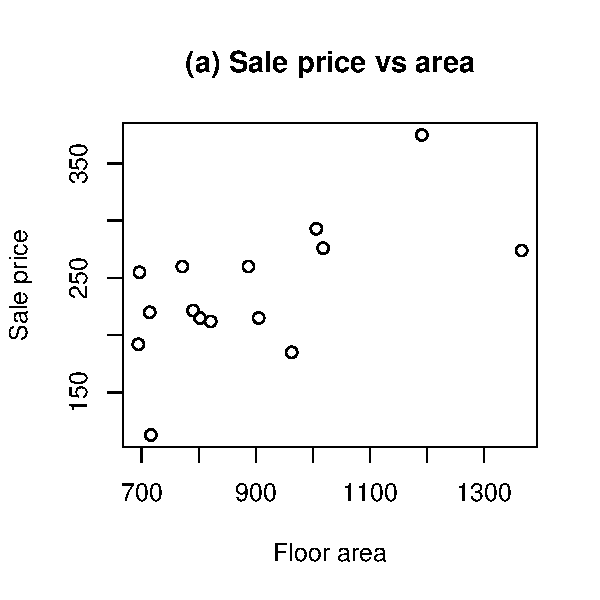
\includegraphics[width=\maxwidth]{figure/unnamed-chunk-12} 

}



\end{knitrout}

\item Use the \verb`hist()` command to plot a histogram of the sale prices
\begin{knitrout}
\definecolor{shadecolor}{rgb}{0.969, 0.969, 0.969}\color{fgcolor}\begin{kframe}
\begin{alltt}
\hlkwd{hist}\hlstd{(houseprices}\hlopt{$}\hlstd{sale.price)}
\end{alltt}
\end{kframe}

{\centering 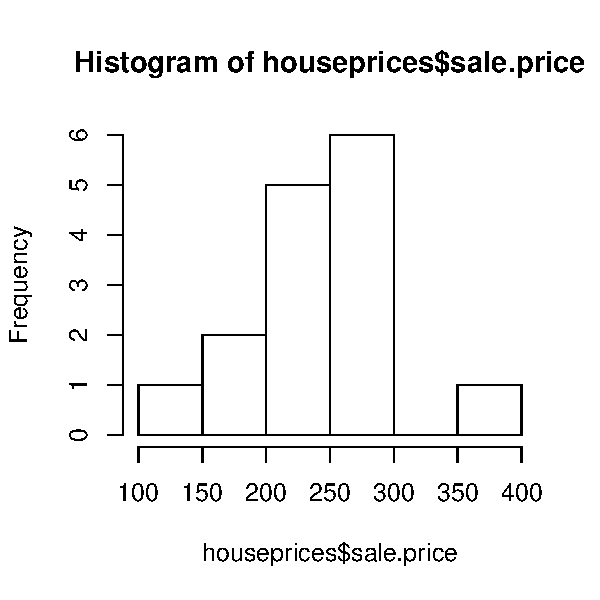
\includegraphics[width=\maxwidth]{figure/unnamed-chunk-13} 

}



\end{knitrout}

\item The following code demonstrates the use of the
\verb+log="y"+ argument to cause \verb+plot+ to use a logarithmic
scale on the \verb+y+ axis, but with axis tick labels that are
specified in the original units.

The next oneputs a logarithmic scale on the $x$-axis
of the histogram.
\begin{knitrout}
\definecolor{shadecolor}{rgb}{0.969, 0.969, 0.969}\color{fgcolor}\begin{kframe}
\begin{alltt}
\hlkwd{par}\hlstd{(}\hlkwc{mfrow}\hlstd{=}\hlkwd{c}\hlstd{(}\hlnum{1}\hlstd{,} \hlnum{2}\hlstd{))}
\hlkwd{plot}\hlstd{(sale.price} \hlopt{~} \hlstd{area,} \hlkwc{data}\hlstd{=houseprices,} \hlkwc{log}\hlstd{=}\hlstr{"y"}\hlstd{,}
     \hlkwc{pch}\hlstd{=}\hlnum{16}\hlstd{,} \hlkwc{xlab}\hlstd{=}\hlstr{"Floor Area"}\hlstd{,} \hlkwc{ylab}\hlstd{=}\hlstr{"Sale Price"}\hlstd{,}
     \hlkwc{main}\hlstd{=}\hlstr{"(c) log(sale.price) vs area"}\hlstd{)}
\hlkwd{hist}\hlstd{(}\hlkwd{log}\hlstd{(houseprices}\hlopt{$}\hlstd{sale.price),}
     \hlkwc{xlab}\hlstd{=}\hlstr{"Sale Price (logarithmic scale)"}\hlstd{,}
     \hlkwc{main}\hlstd{=}\hlstr{"(c)  Histogram of log(sale.price)"}\hlstd{)}
\end{alltt}
\end{kframe}

{\centering 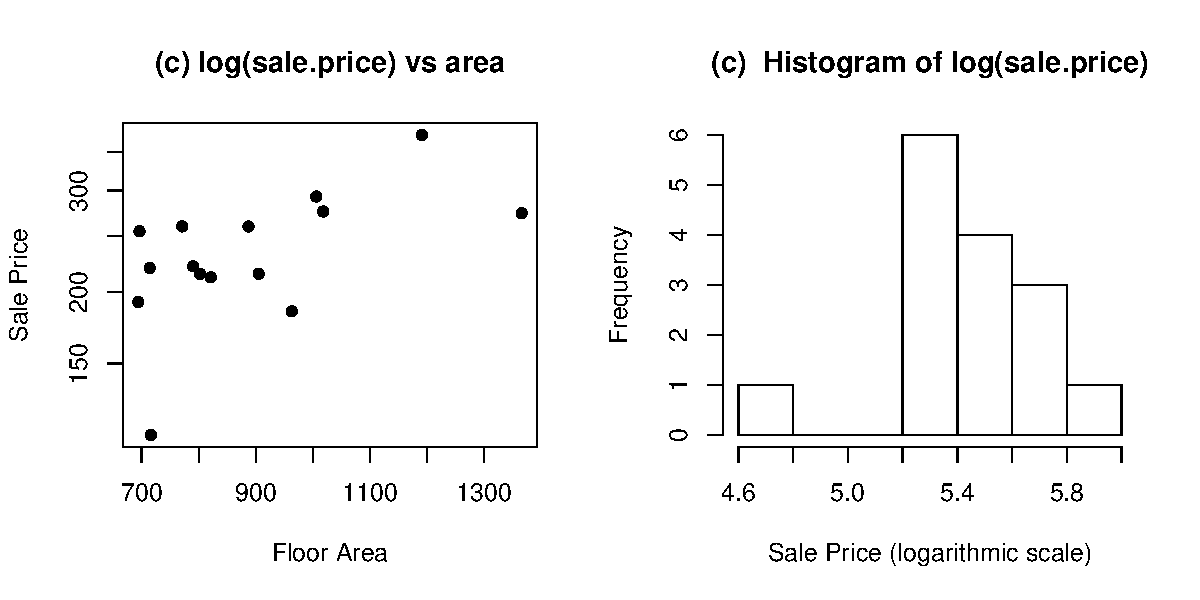
\includegraphics[width=\maxwidth]{figure/unnamed-chunk-14} 

}


\begin{kframe}\begin{alltt}
\hlkwd{par}\hlstd{(}\hlkwc{mfrow}\hlstd{=}\hlkwd{c}\hlstd{(}\hlnum{1}\hlstd{,} \hlnum{1}\hlstd{))}
\end{alltt}
\end{kframe}
\end{knitrout}

\item Compare the two histograms

\begin{knitrout}
\definecolor{shadecolor}{rgb}{0.969, 0.969, 0.969}\color{fgcolor}\begin{kframe}
\begin{alltt}
\hlkwd{par}\hlstd{(}\hlkwc{mfrow}\hlstd{=}\hlkwd{c}\hlstd{(}\hlnum{1}\hlstd{,} \hlnum{2}\hlstd{))}
\hlkwd{hist}\hlstd{(houseprices}\hlopt{$}\hlstd{sale.price,}
     \hlkwc{xlab}\hlstd{=}\hlstr{"Sale Price"}\hlstd{,}
     \hlkwc{main}\hlstd{=}\hlstr{"Histogram of sale.price"}\hlstd{)}
\hlkwd{hist}\hlstd{(}\hlkwd{log}\hlstd{(houseprices}\hlopt{$}\hlstd{sale.price),}
     \hlkwc{xlab}\hlstd{=}\hlstr{"Sale Price (logarithmic scale)"}\hlstd{,}
     \hlkwc{main}\hlstd{=}\hlstr{"Histogram of log(sale.price)"}\hlstd{)}
\end{alltt}
\end{kframe}

{\centering 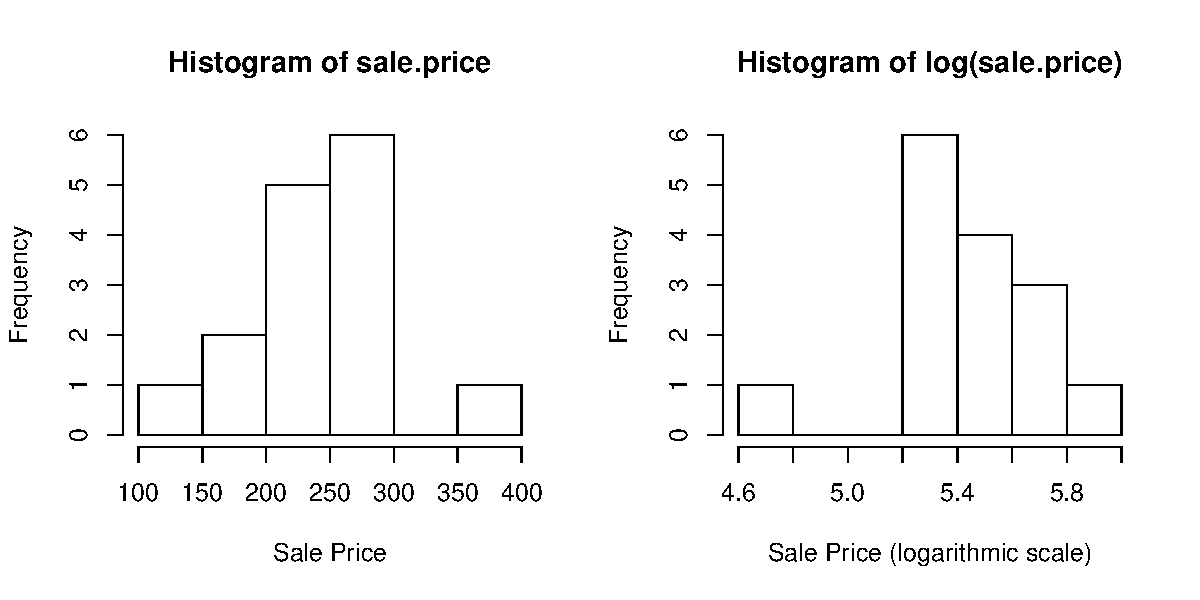
\includegraphics[width=\maxwidth]{figure/unnamed-chunk-15} 

}


\begin{kframe}\begin{alltt}
\hlkwd{par}\hlstd{(}\hlkwc{mfrow}\hlstd{=}\hlkwd{c}\hlstd{(}\hlnum{1}\hlstd{,} \hlnum{1}\hlstd{))}
\end{alltt}
\end{kframe}
\end{knitrout}
\end{enumerate}

At log scale, the small difference (i.e. to the left of the axis) is indistinguisable. The log scale emphasizes the larger spread. To see this more clearly, consider the following plot:

\begin{knitrout}
\definecolor{shadecolor}{rgb}{0.969, 0.969, 0.969}\color{fgcolor}\begin{kframe}
\begin{alltt}
\hlkwd{plot}\hlstd{(}\hlkwd{log}\hlstd{(}\hlkwd{seq}\hlstd{(}\hlnum{100}\hlopt{:}\hlnum{400}\hlstd{)),} \hlkwc{type}\hlstd{=}\hlstr{"l"}\hlstd{,} \hlkwc{ylab}\hlstd{=}\hlstr{"log_sale_price"}\hlstd{,} \hlkwc{xlab}\hlstd{=}\hlstr{"sale_price"}\hlstd{)}
\hlkwd{abline}\hlstd{(}\hlkwc{v}\hlstd{=}\hlkwd{exp}\hlstd{(}\hlnum{2}\hlstd{),} \hlkwc{col}\hlstd{=}\hlstr{"red"}\hlstd{)}
\hlkwd{abline}\hlstd{(}\hlkwc{v}\hlstd{=}\hlkwd{exp}\hlstd{(}\hlnum{3}\hlstd{),} \hlkwc{col}\hlstd{=}\hlstr{"red"}\hlstd{)}
\hlkwd{abline}\hlstd{(}\hlkwc{v}\hlstd{=}\hlkwd{exp}\hlstd{(}\hlnum{4}\hlstd{),} \hlkwc{col}\hlstd{=}\hlstr{"blue"}\hlstd{)}
\hlkwd{abline}\hlstd{(}\hlkwc{v}\hlstd{=}\hlkwd{exp}\hlstd{(}\hlnum{5}\hlstd{),} \hlkwc{col}\hlstd{=}\hlstr{"blue"}\hlstd{)}
\end{alltt}
\end{kframe}

{\centering 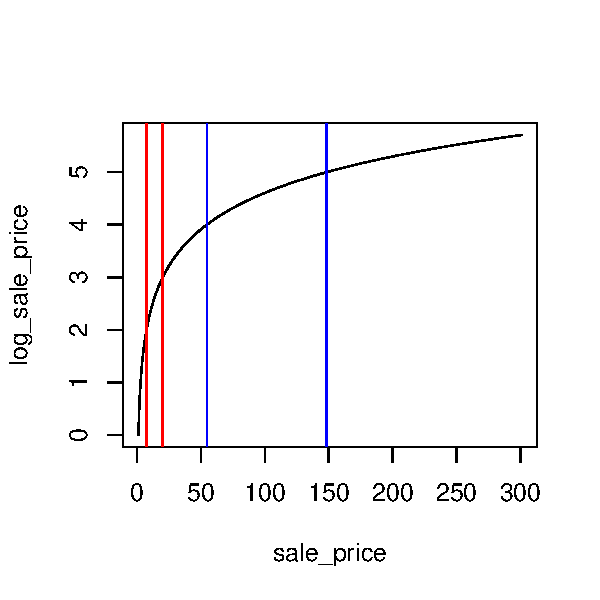
\includegraphics[width=\maxwidth]{figure/unnamed-chunk-16} 

}



\end{knitrout}

Notice that one unit increase in \verb`log_sale_price` does not correspond with the same increase in \verb`sale_price`. For example, \verb`log_sale_price` increases from 2 to 3 between the red lines, and from 4 to 5 between the blue lines (an increase of 1 in both cases). However, the change of \verb`sale_price` between the blue lines is much greater than between the red lines. More generally, the farther we are to the right, the larger 1 unit in log scale becomes.

Back to our original question, this means that to the right of our log scale histogram, one unit in the x axis covers a lot more houses. Thus, the histogram is higher to the right.
\end{document}
